% Standard Article Definition
\documentclass[]{article}

% Page Formatting
\usepackage[margin=1in]{geometry}
\setlength\parindent{0pt}

% Graphics
\usepackage{graphicx}

% Math Packages
\usepackage{physics}
\usepackage{amsmath, amsfonts, amssymb, amsthm}
\usepackage{mathtools}

% Extra Packages
\usepackage{pdfpages}
\usepackage{hyperref}
% \usepackage{listings}

% Section Heading Settings
% \usepackage{enumitem}
% \renewcommand{\theenumi}{\alph{enumi}}
\renewcommand*{\thesection}{Problem \arabic{section}}
\renewcommand*{\thesubsection}{\arabic{section}\alph{subsection})}
\renewcommand*{\thesubsubsection}{}%\quad \quad \roman{subsubsection})}

\newcommand{\Problem}{\subsubsection*{\textbf{PROBLEM:}}}
\newcommand{\Solution}{\subsubsection*{\textbf{SOLUTION:}}}
\newcommand{\Preliminaries}{\subsubsection*{\textbf{PRELIMINARIES:}}}

%Custom Commands
\newcommand{\N}{\mathbb{N}}
\newcommand{\Z}{\mathbb{Z}}
% \newcommand{\Q}{\mathbb{Q}}
\newcommand{\R}{\mathbb{R}}
\newcommand{\C}{\mathbb{C}}

% \newcommand{\SigAlg}{\mathcal{S}}

% \newcommand{\Rel}{\mathcal{R}}

% \newcommand{\toI}{\xrightarrow{\textsf{\tiny I}}}
% \newcommand{\toS}{\xrightarrow{\textsf{\tiny S}}}
% \newcommand{\toB}{\xrightarrow{\textsf{\tiny B}}}

% \newcommand{\divisible}{ \ \vdots \ }
\newcommand{\st}{\ : \ }

% Theorem Definition
\newtheorem{definition}{Definition}
\newtheorem{assumption}{Assumption}
\newtheorem{theorem}{Theorem}
\newtheorem{lemma}{Lemma}
\newtheorem{proposition}{Proposition}
\newtheorem{remark}{Remark}
% \newtheorem{example}{Example}
% \newtheorem{counterExample}{Counter Example}


%opening
\title{
    MECH 6v29 - Model Predictive Control\\ 
    Homework 2
}
\author{Jonas Wagner\\ jonas.wagner@utdallas.edu}
\date{2023, September 29\textsuperscript{th}}

\begin{document}

\maketitle

\tableofcontents

%% Problem 1
\newpage
\section{}

% 1a)
\subsection{}

\begin{figure}[h]
    \centering
    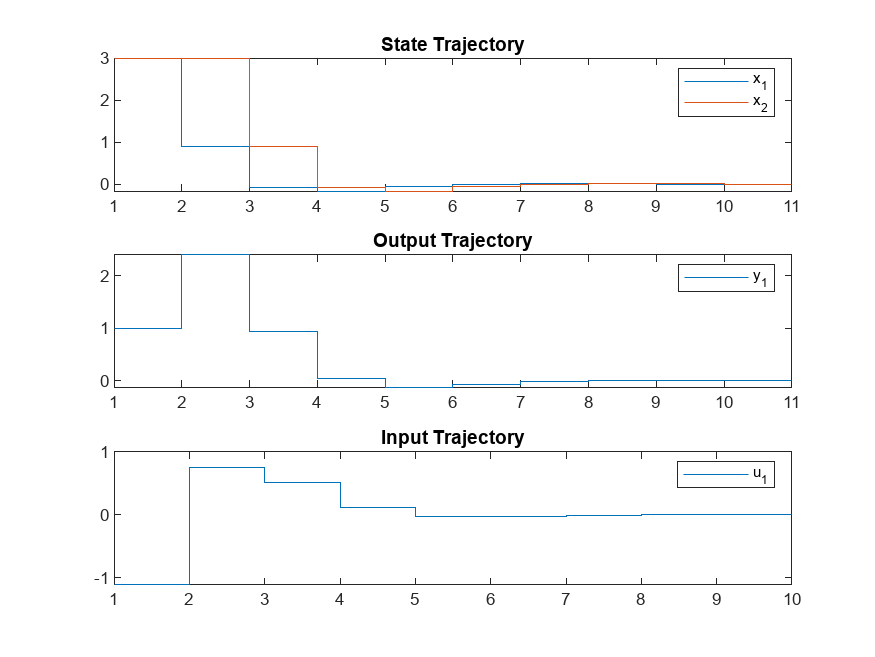
\includegraphics[width = 0.5\textwidth]{figs/pblm1a.png}
    \caption{Problem 1a results}
\end{figure}

The transient behavior is pretty reasonable and has a mild overshoot.
The maximum output is around 2.5 (2.409) and it appears to initially reach the origin after 4 timesteps but takes around 7 to settle.

% 1b)
\newpage
\subsection{}
\begin{figure}[h]
    \centering
    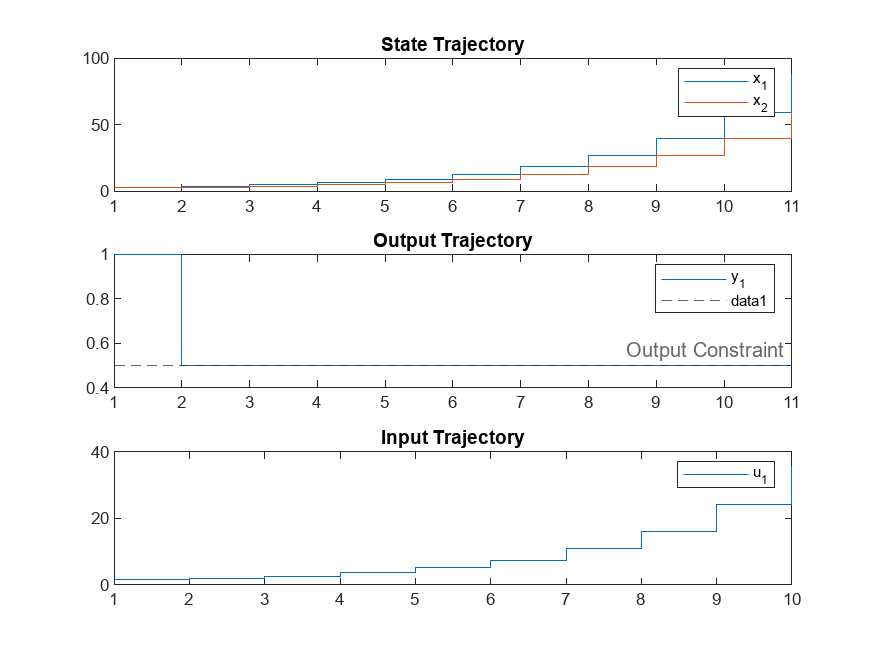
\includegraphics[width = 0.5\textwidth]{figs/pblm1b.png}
    \caption{Problem 1b results}
\end{figure}

The controller is unable to stabilize the system.

Is it possible to tune the cost function matrices? 
Potentially, although I'm not sure how to explicitly prove this either way for every case that this controller would face.
I did test multiple versions of the matrices but did not find any that satisfied it.

% 1c)
\newpage
\subsection{}
The first time step ``solution'' is 0.
Looking at error code we find that the controller result is actually is infeasible or unbounded.

After it runs for a couple time steps with $u=0$, it then becomes feasible and has a solution that ultimately does stabilize the system.

\begin{figure}[h]
    \centering
    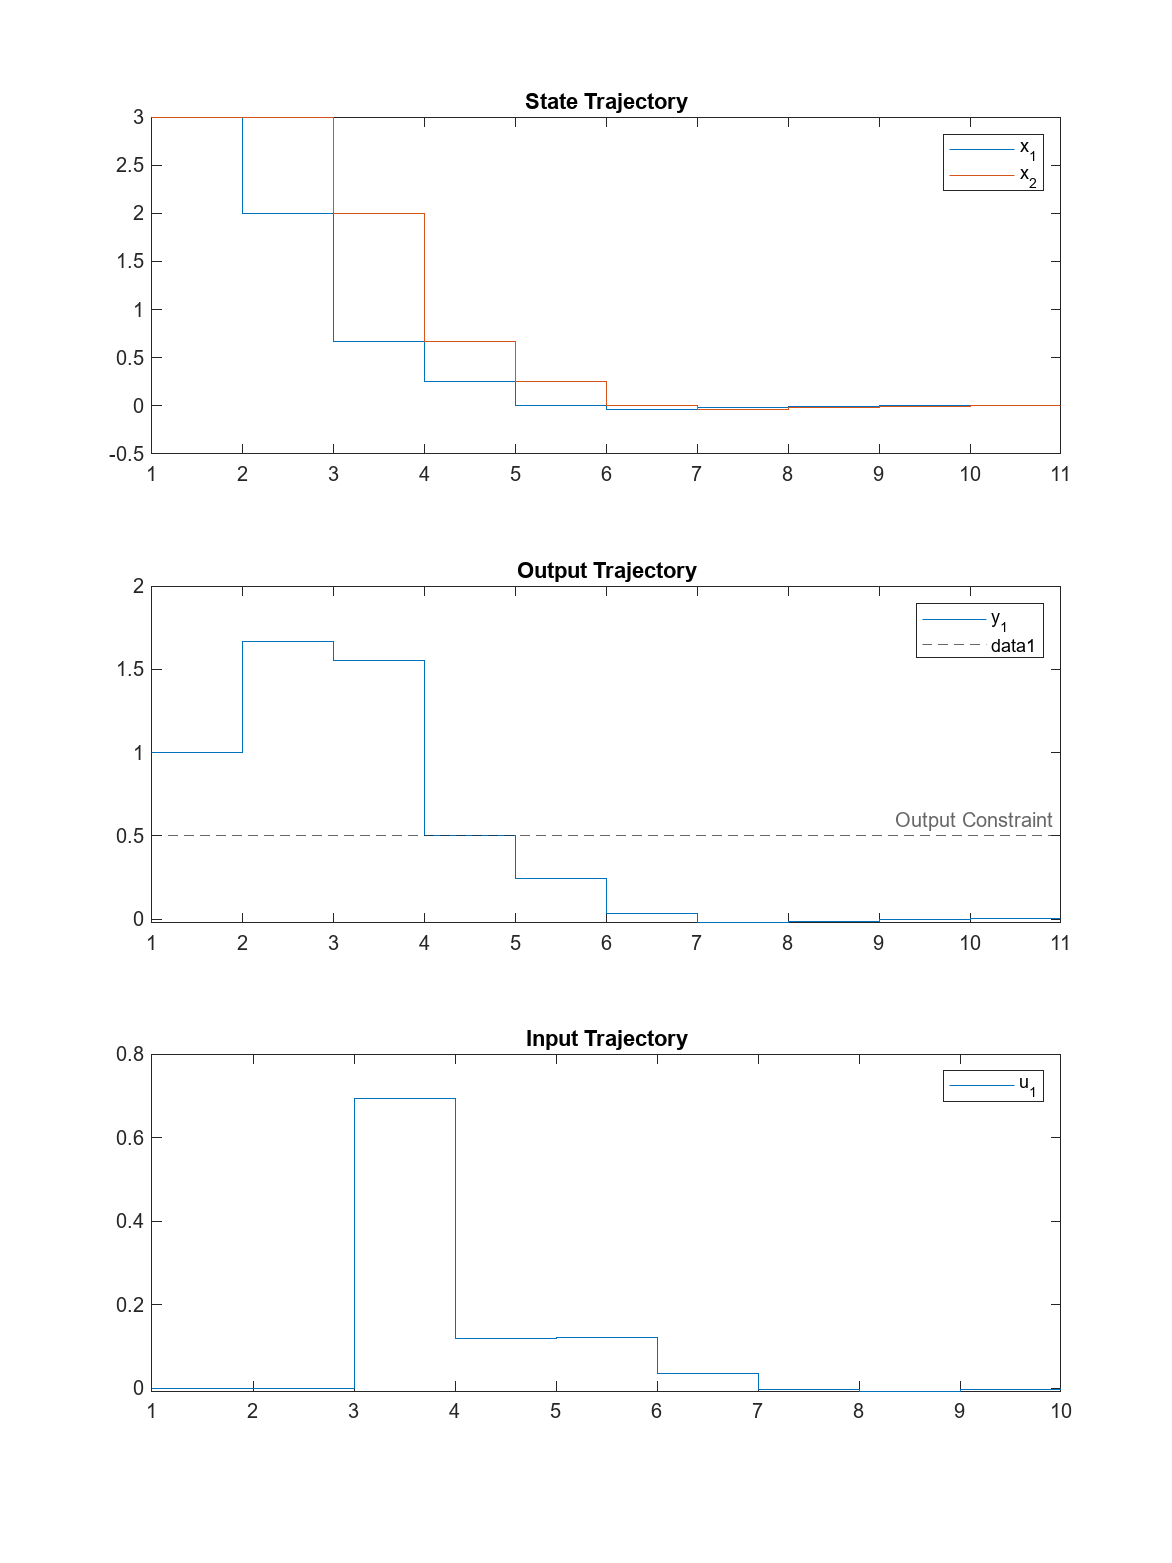
\includegraphics[width = 0.5\textwidth]{figs/pblm1c.png}
    \caption{Problem 1c results}
\end{figure}

Increasing the time does not appear to solve this issue.
Specifically, increasing it incrementally up to 10 saw no difference, and then running it at $N=50$ also demonstrated no changes.

% 1d)
\newpage
\subsection{}
% \begin{figure}[h]
%     \centering
%     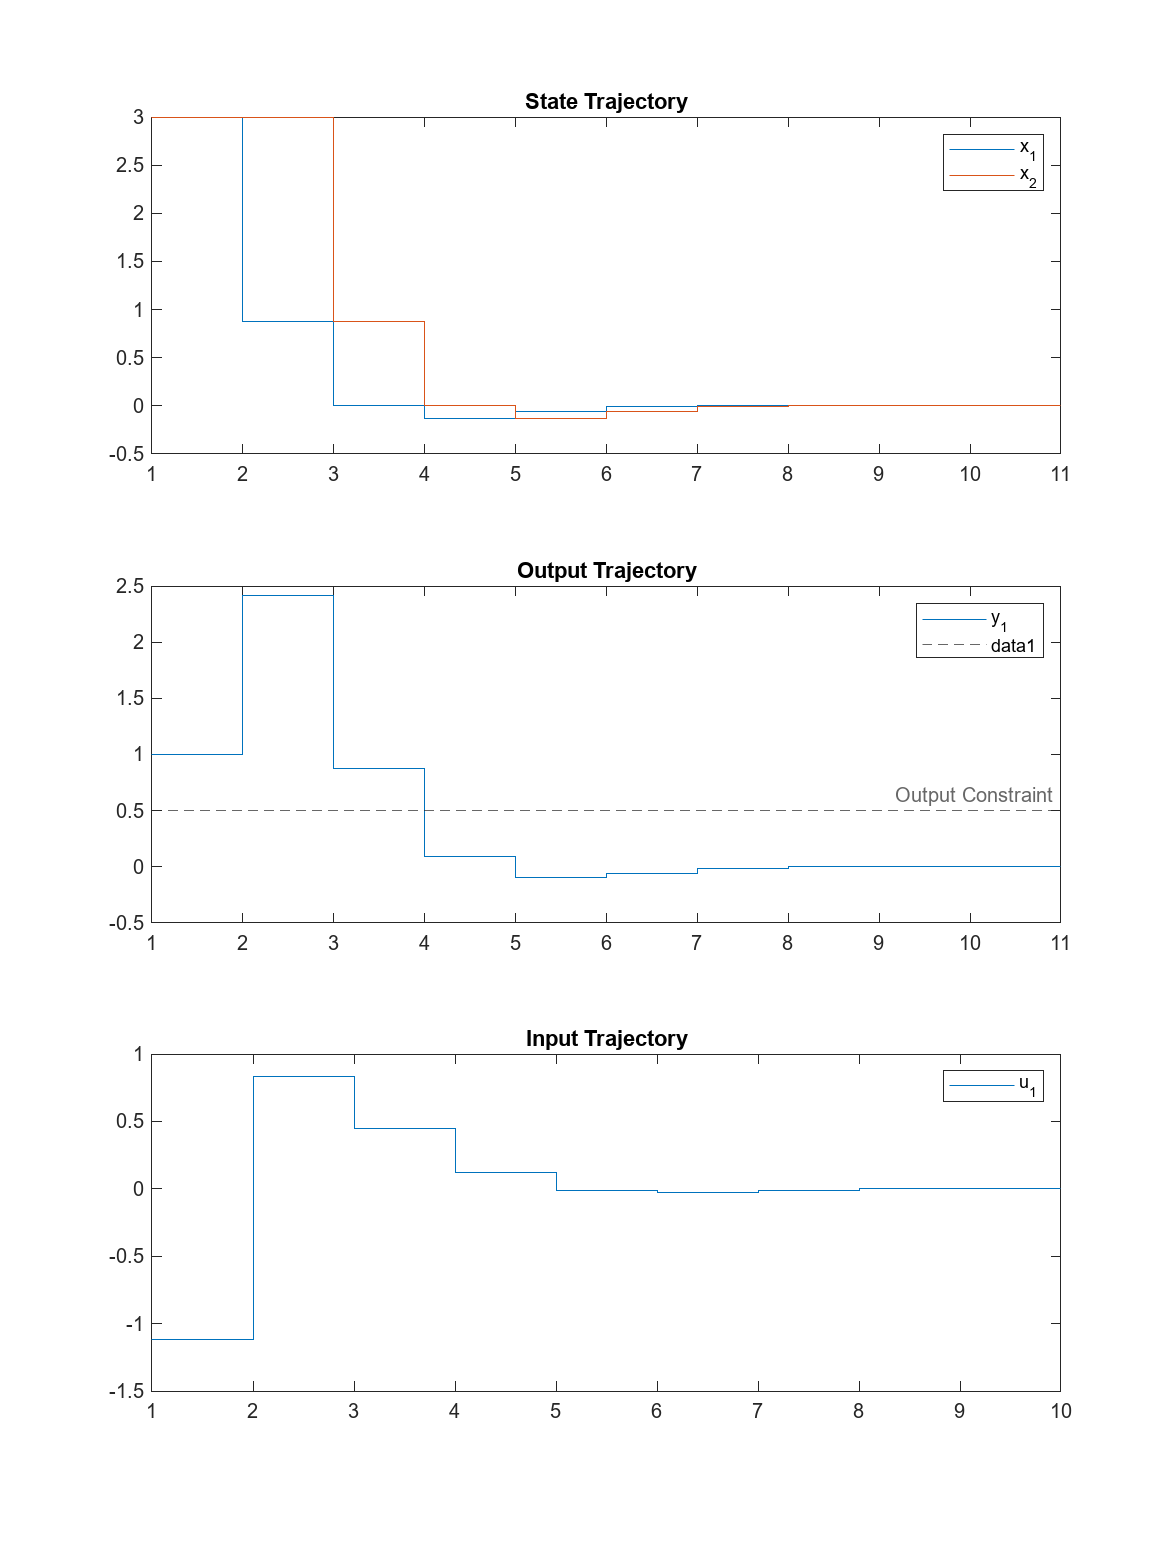
\includegraphics[width = 0.5\textwidth]{figs/pblm1d.png}
%     \caption{Problem 1d initial results (just w/ a slack variable)}
% \end{figure}

I ran this for many different time-horrizons (and the slack variable was weighted with a gain of 100).
A few of these are included here (the rest available on github).
Essential takeaway is that the extension of time-horizon allows for a less extreme peak output value and longer period that the output constraint is maintained.
Additionally, the specific note of combining the two is that feasibility becomes a much larger concern but at a minimum, the constraint at $x_N = 0$ ensures stability (although a slack variable should also be added to ensure feasibility).

\begin{figure}[h]
    \centering
    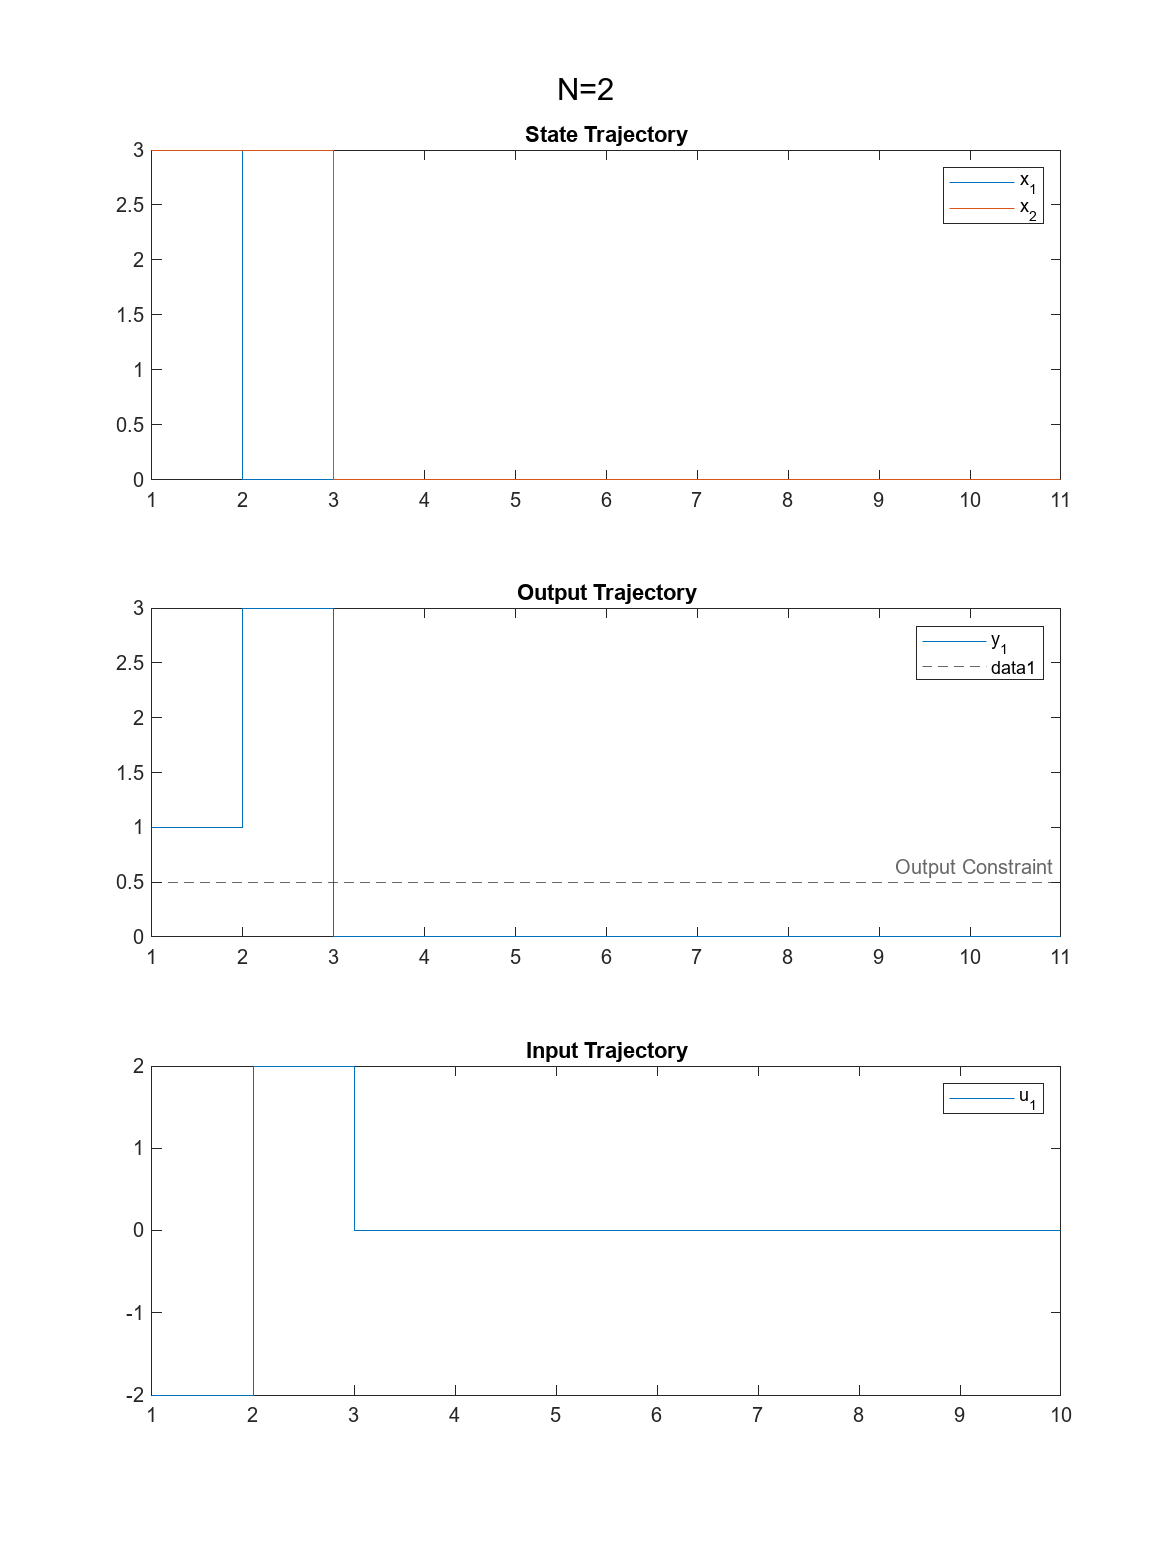
\includegraphics[width=0.3\textwidth]{figs/pblm1d_N=2.png}
    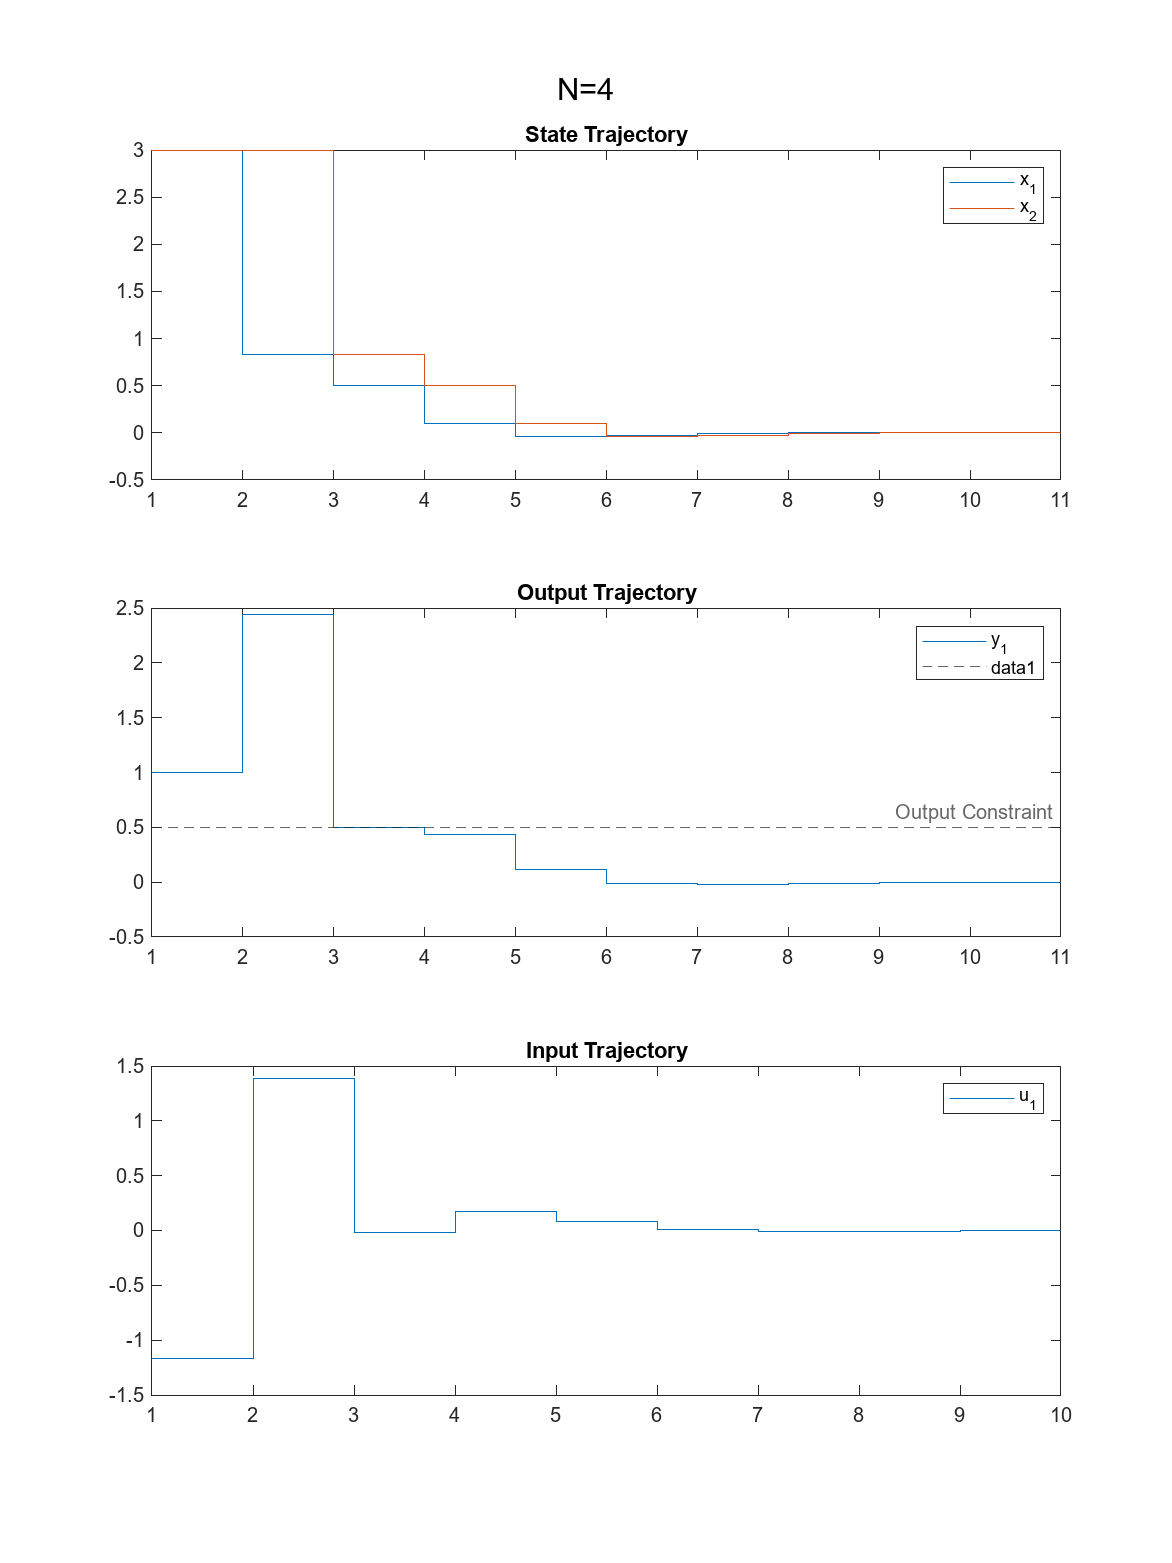
\includegraphics[width=0.3\textwidth]{figs/pblm1d_N=4.png}
    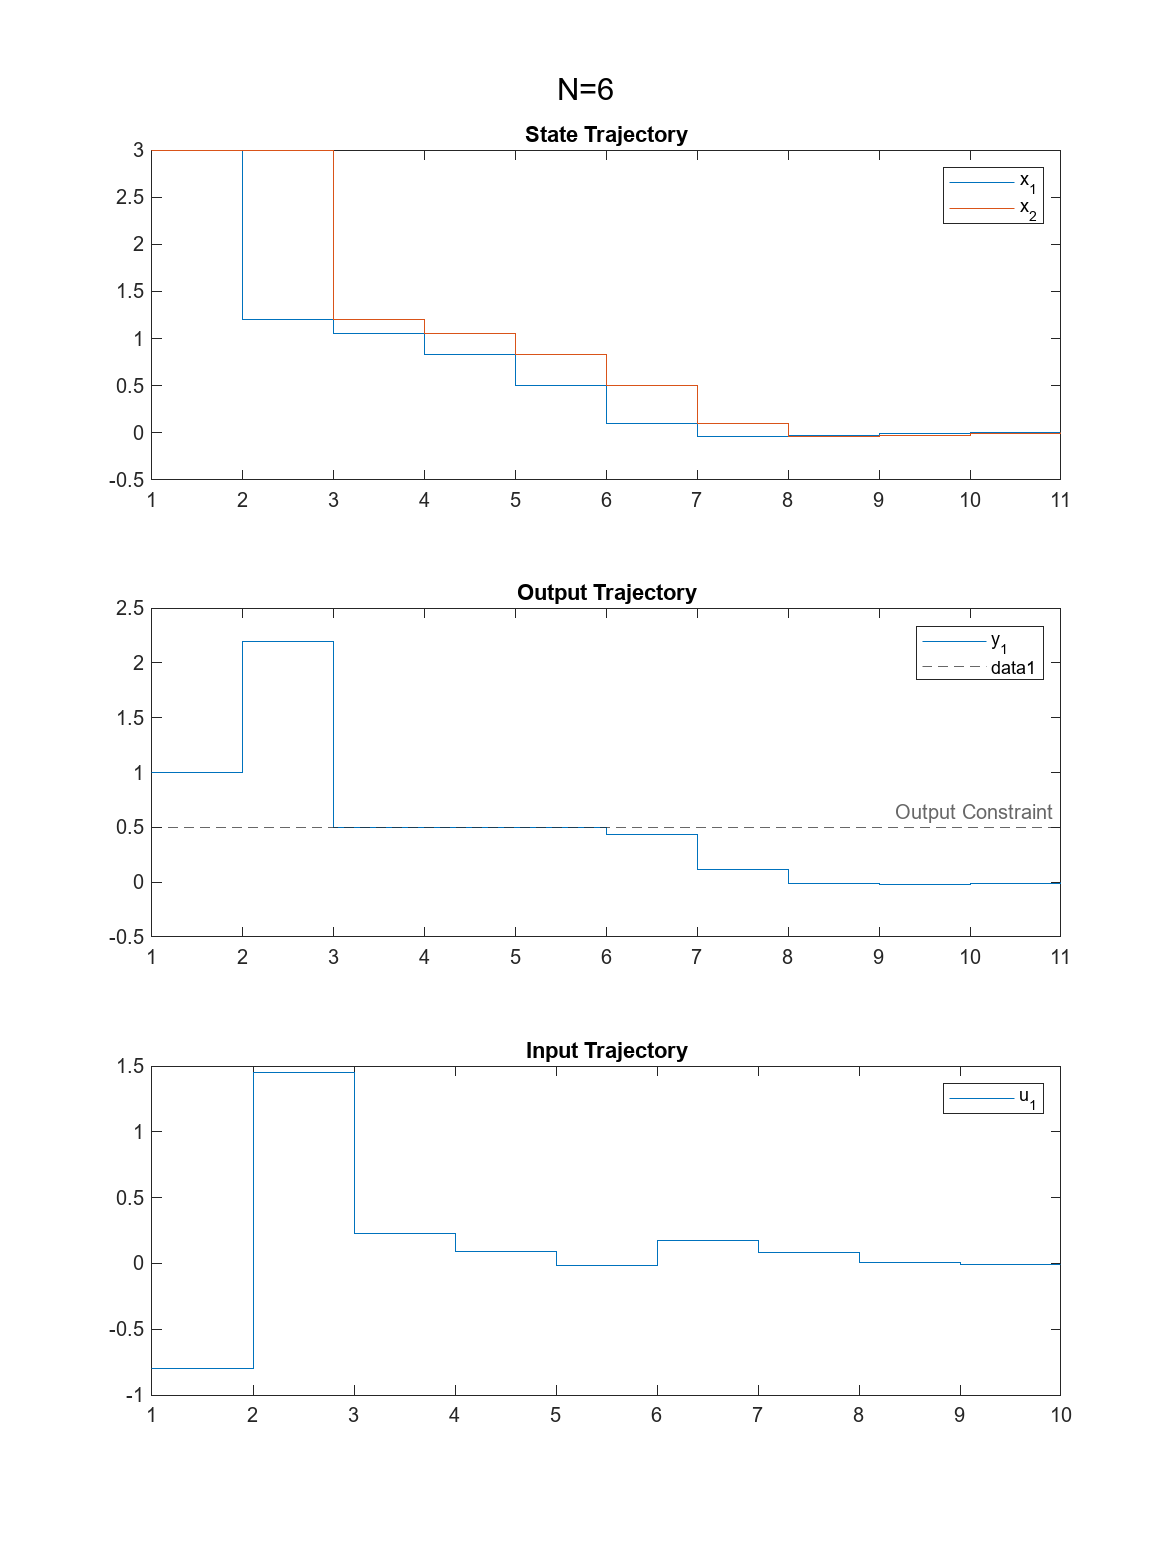
\includegraphics[width=0.3\textwidth]{figs/pblm1d_N=6.png}
    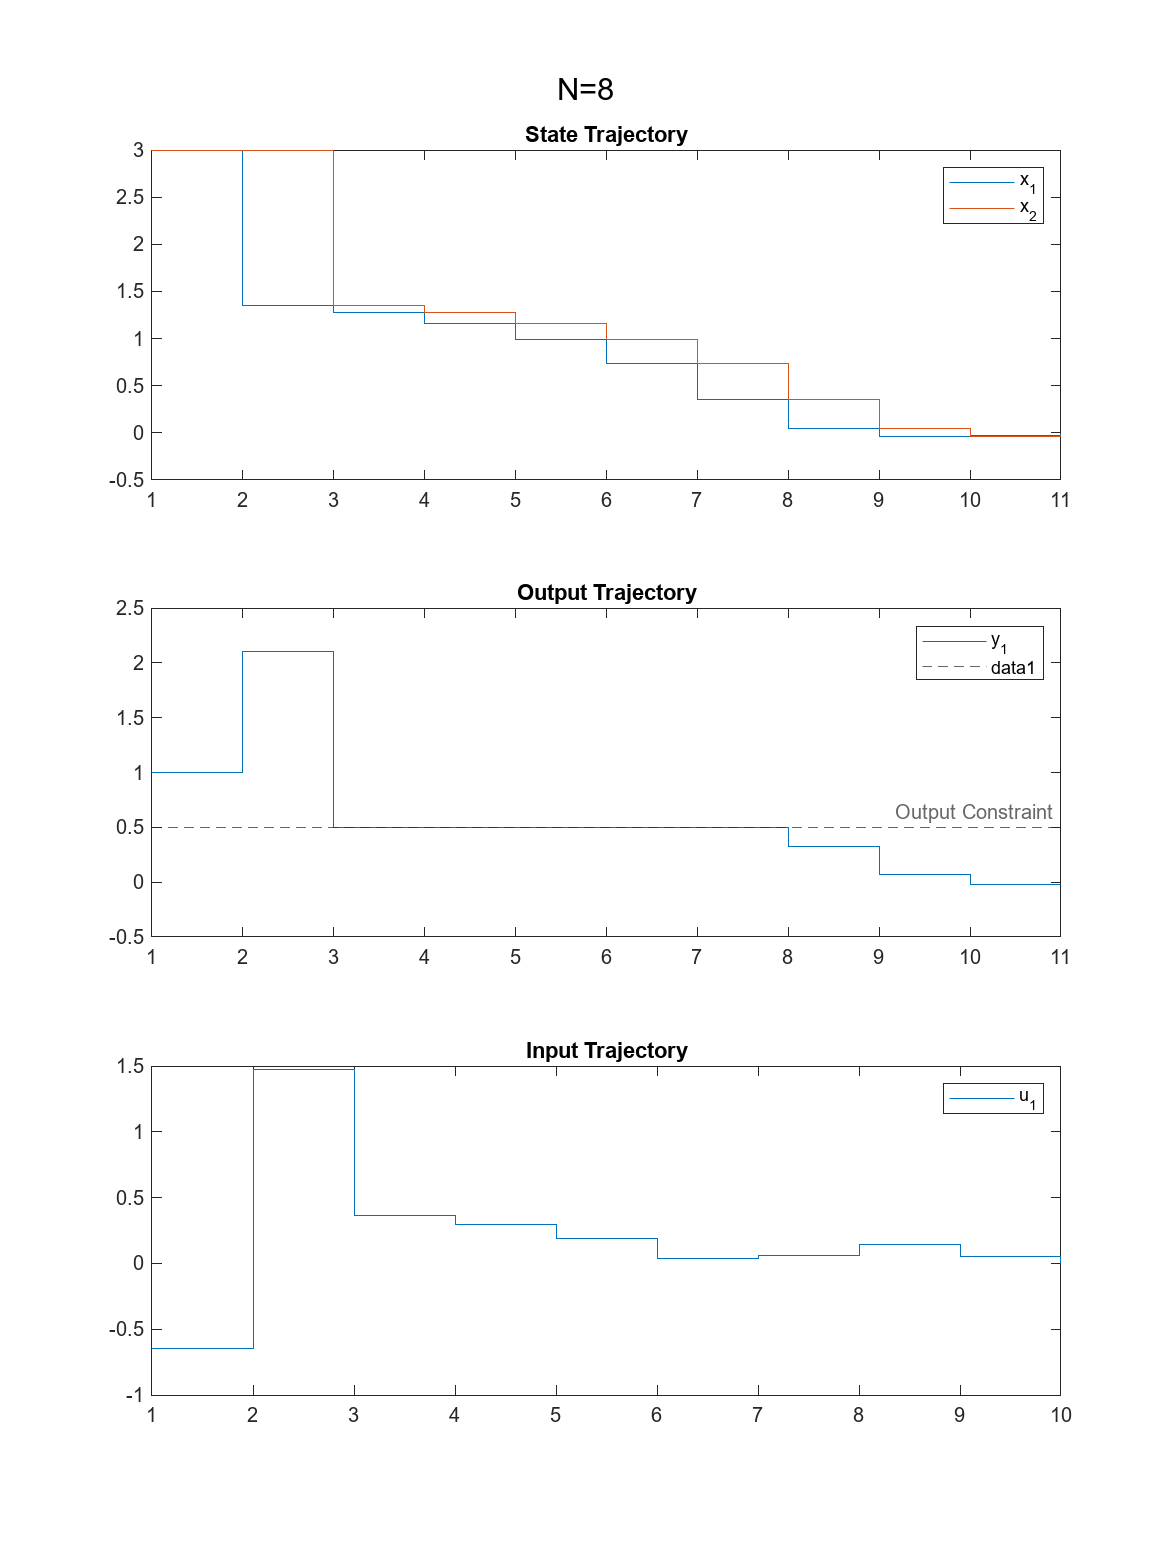
\includegraphics[width=0.3\textwidth]{figs/pblm1d_N=8.png}
    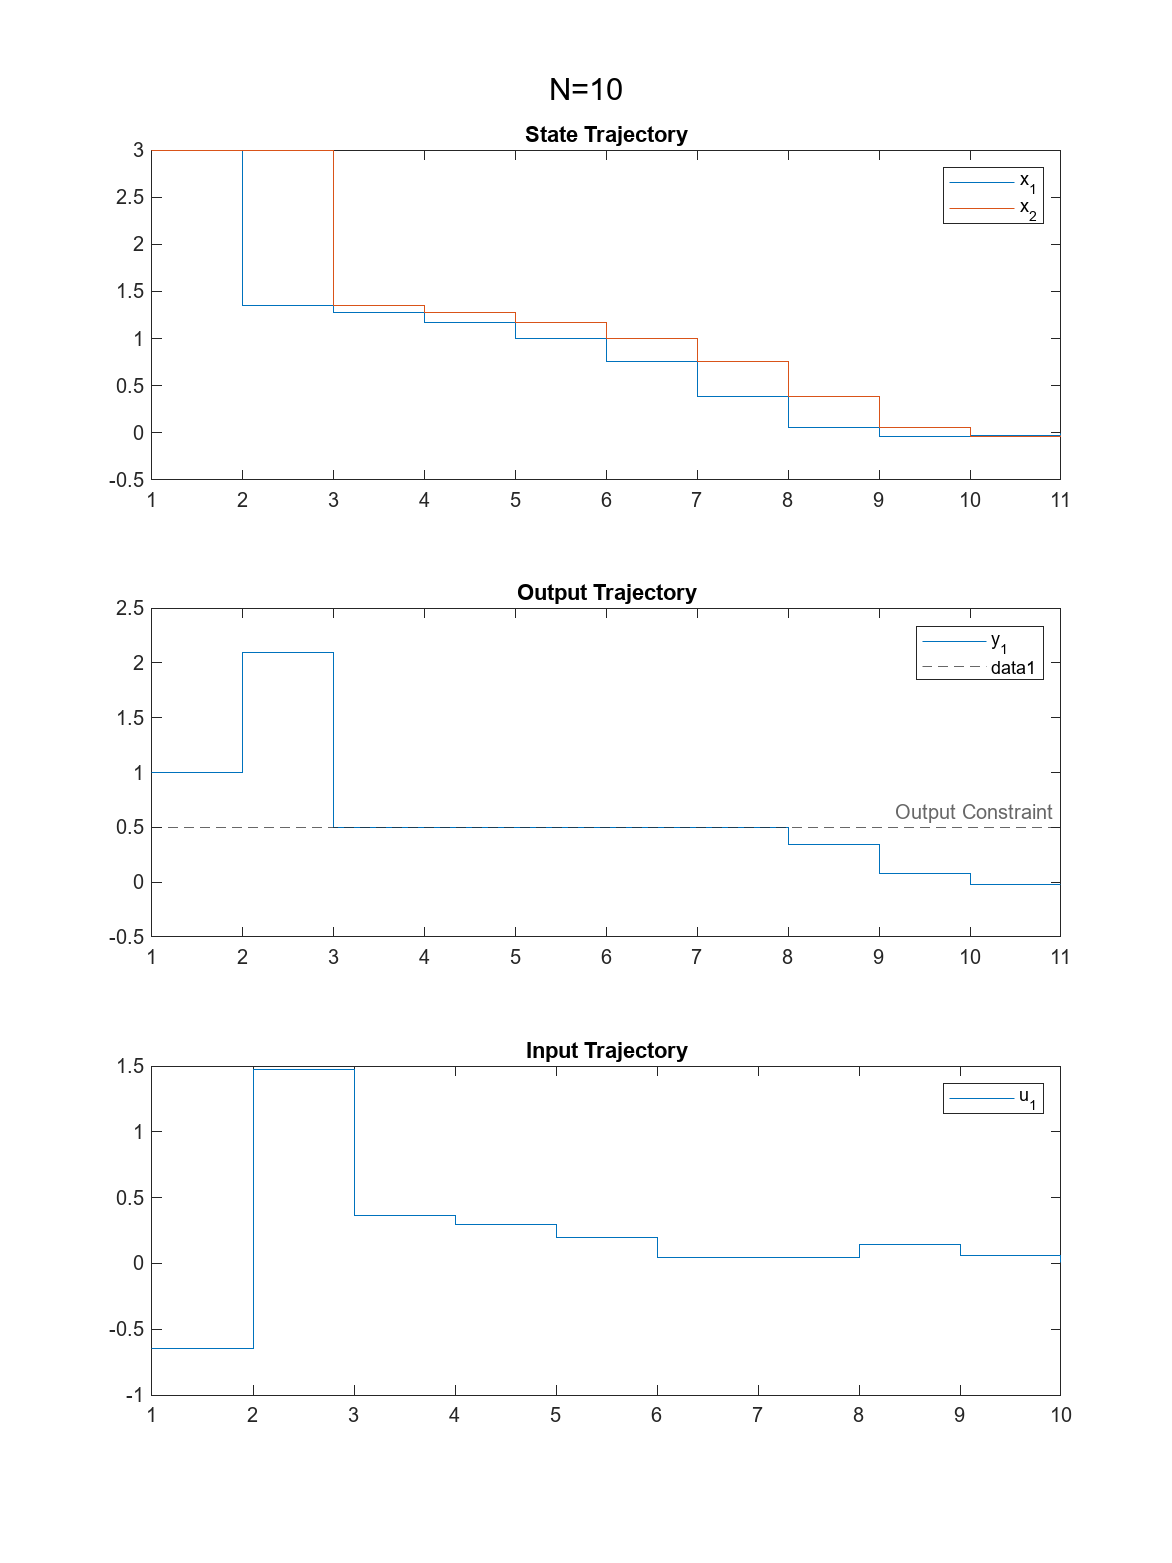
\includegraphics[width=0.3\textwidth]{figs/pblm1d_N=10.png}
    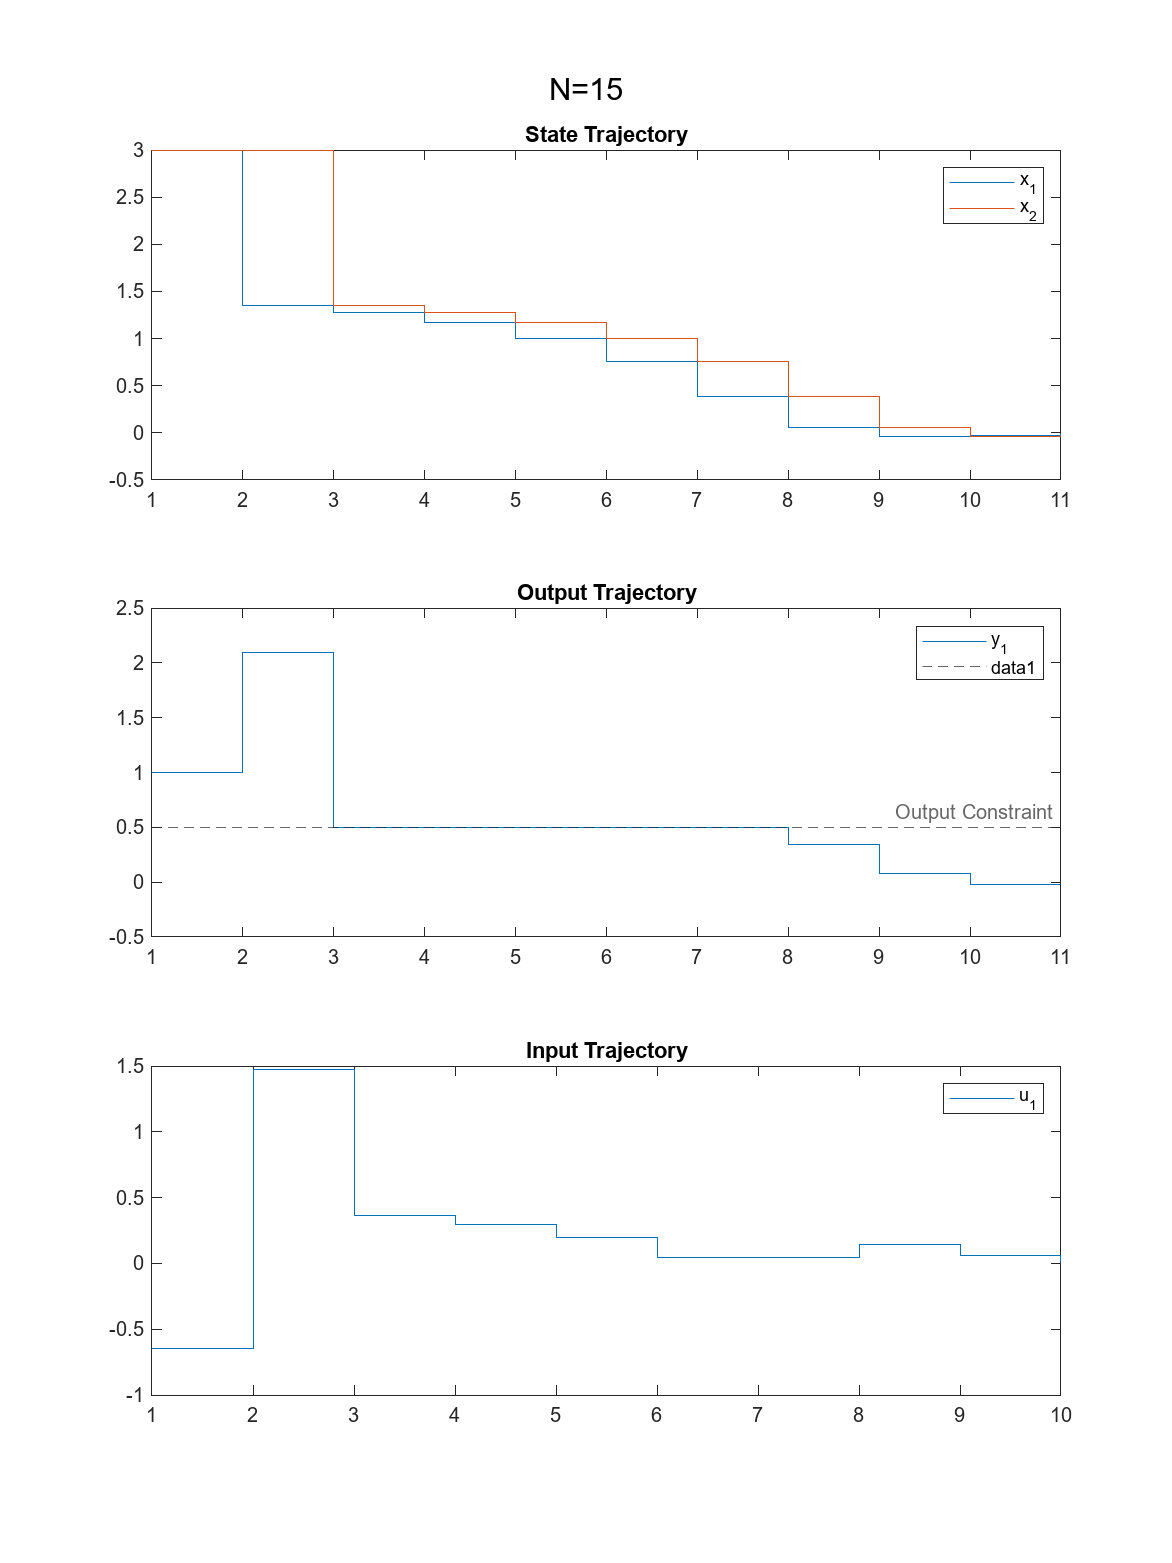
\includegraphics[width=0.3\textwidth]{figs/pblm1d_N=15.png}
\end{figure}

\newpage

%% Problem 2
\newpage
\section{}
\[
    A = \mqty[2&1\\0&2] \quad B = \mqty[1&0\\0&1]
\]\[
    \mathcal{X} = \{x \in \R^2 \st \mqty[1&0] x \leq 5\}
\]\[
    \mathcal{U} = \{u \in \R^2 \st -\vb{1} \leq u \leq \vb{1}\}
\]
Note: $\mathcal{X} = \{x \in \R^2 \st x_1 \leq 5\}$ 
and $\mathcal{U} = \{u \in \R^2 \st \norm{u}_{\infty} \leq 1\}$

Or (in H-rep) $\mathcal{X} = \{\mqty[1&0], 5\}$ 
and $\mathcal{U} = \{\mqty[\vb{I}_2\\-\vb{I}_2], \mqty[\vb{1}_2\\\vb{1}_2]\}$

% 2a)
\subsection{}
Running it for many different values of alpha resulted in the following:

\begin{figure}[h]
    \centering
    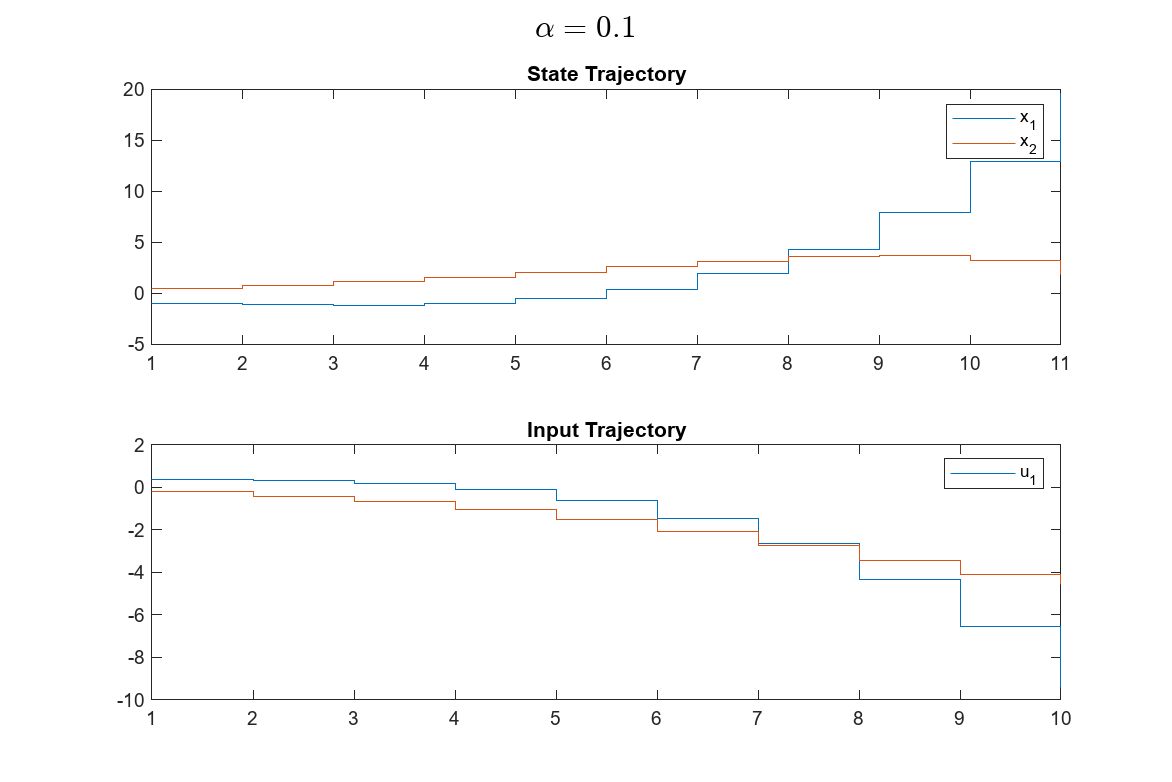
\includegraphics[width=0.3\textwidth]{figs/pblm2a_alpha=1e-01.png}
    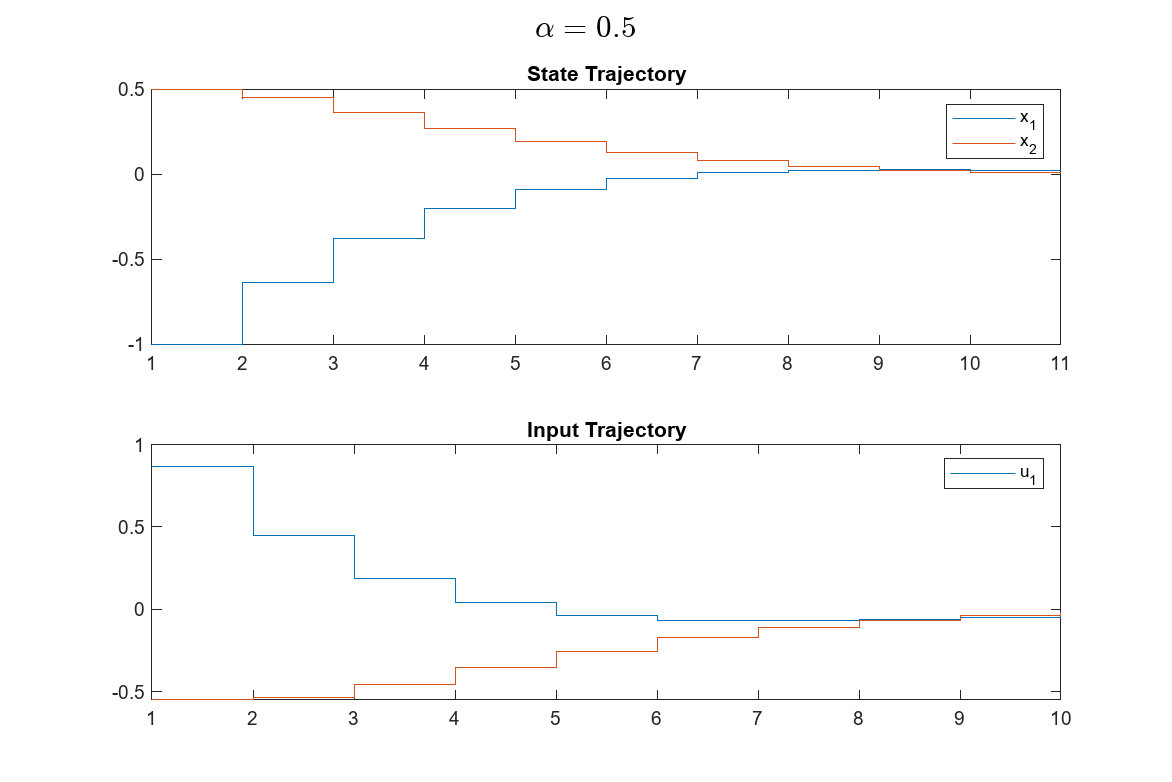
\includegraphics[width=0.3\textwidth]{figs/pblm2a_alpha=5e-01.png}
    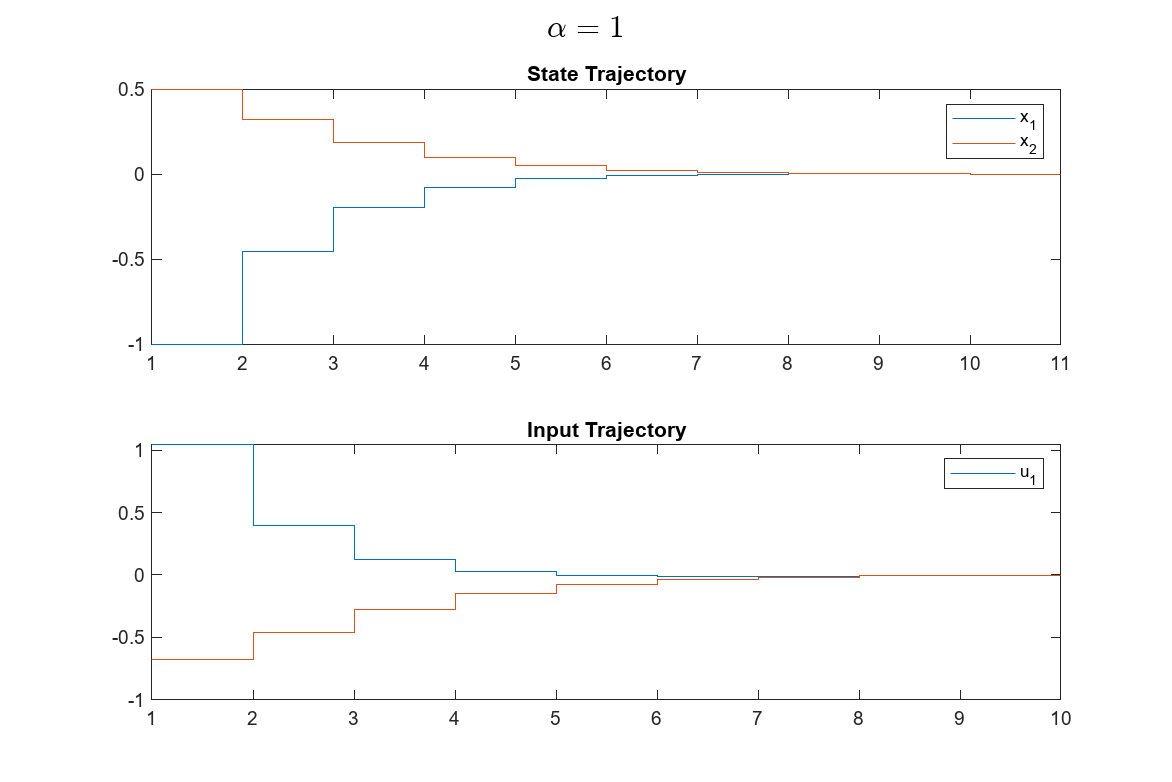
\includegraphics[width=0.3\textwidth]{figs/pblm2a_alpha=1e+00.png}
    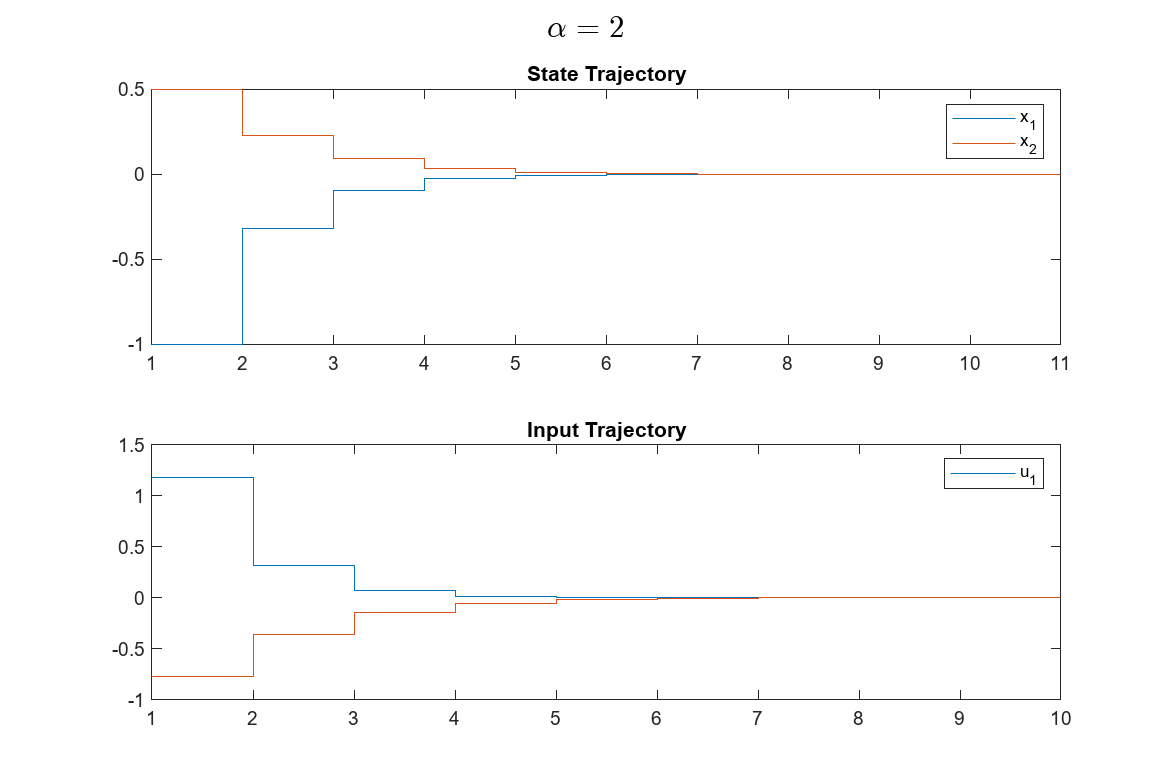
\includegraphics[width=0.3\textwidth]{figs/pblm2a_alpha=2e+00.png}
    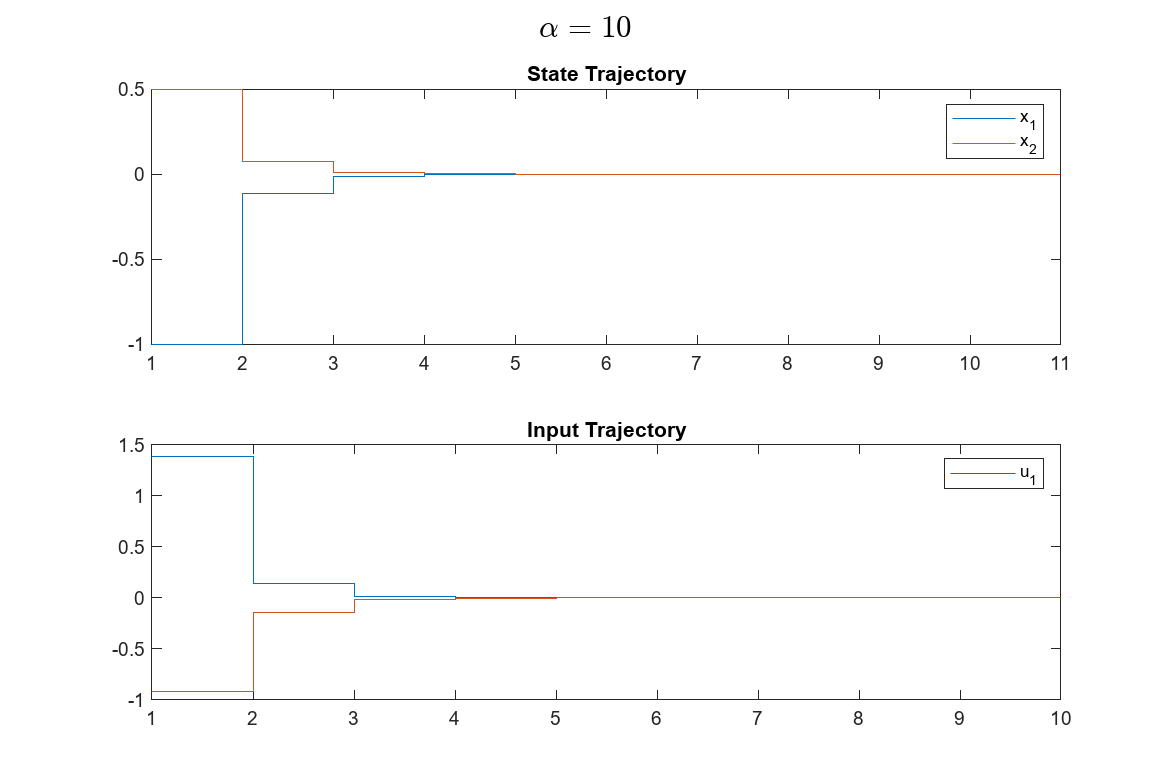
\includegraphics[width=0.3\textwidth]{figs/pblm2a_alpha=1e+01.png}
\end{figure}
When $\alpha = 0.1$ the system is unstable.

% 2b)
\newpage
\subsection{}
When implementing the state and input constraints, the closed loop system is still unstable.
\begin{figure}[h]
    \centering
    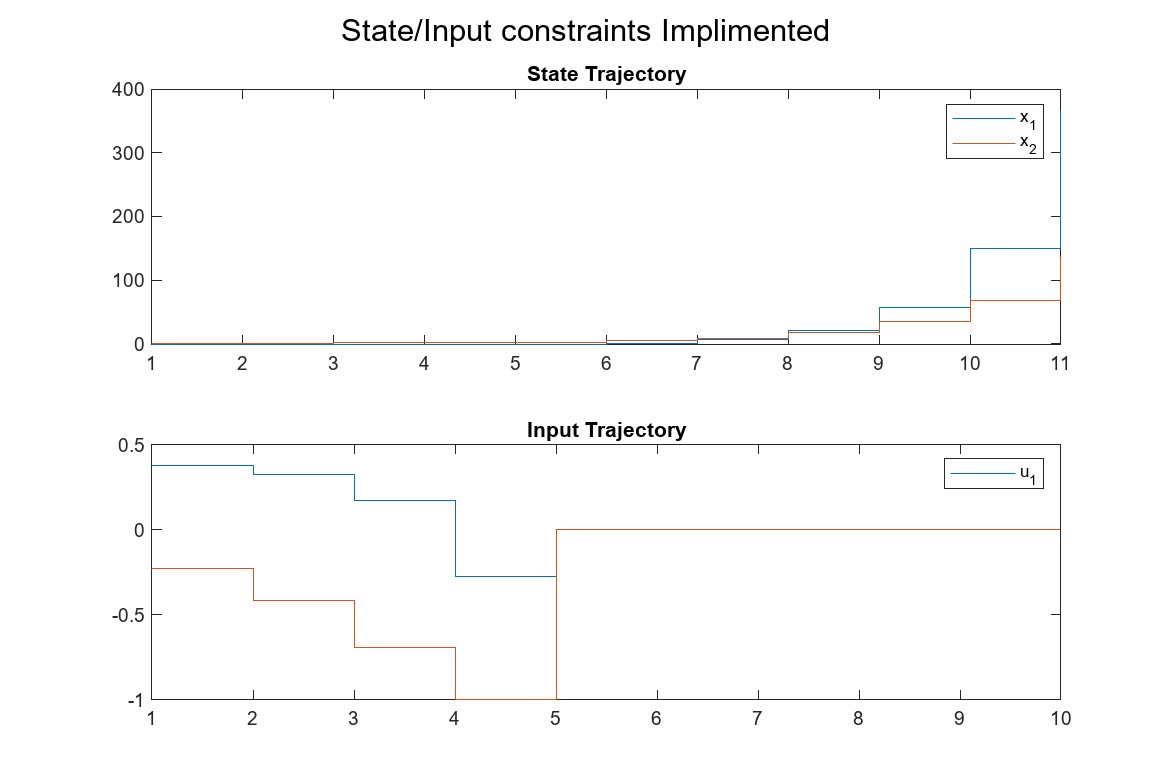
\includegraphics[width=0.7\textwidth]{figs/pblm2b}
\end{figure}
Additionally, the results become infeasible once it diverges from the origin too much.

% 2c)
\newpage
\subsection{}
Implementing it with the $x_N = 0$ constraint allows it to be stable (and feasibility issues disappear).
\begin{figure}[h]
    \centering
    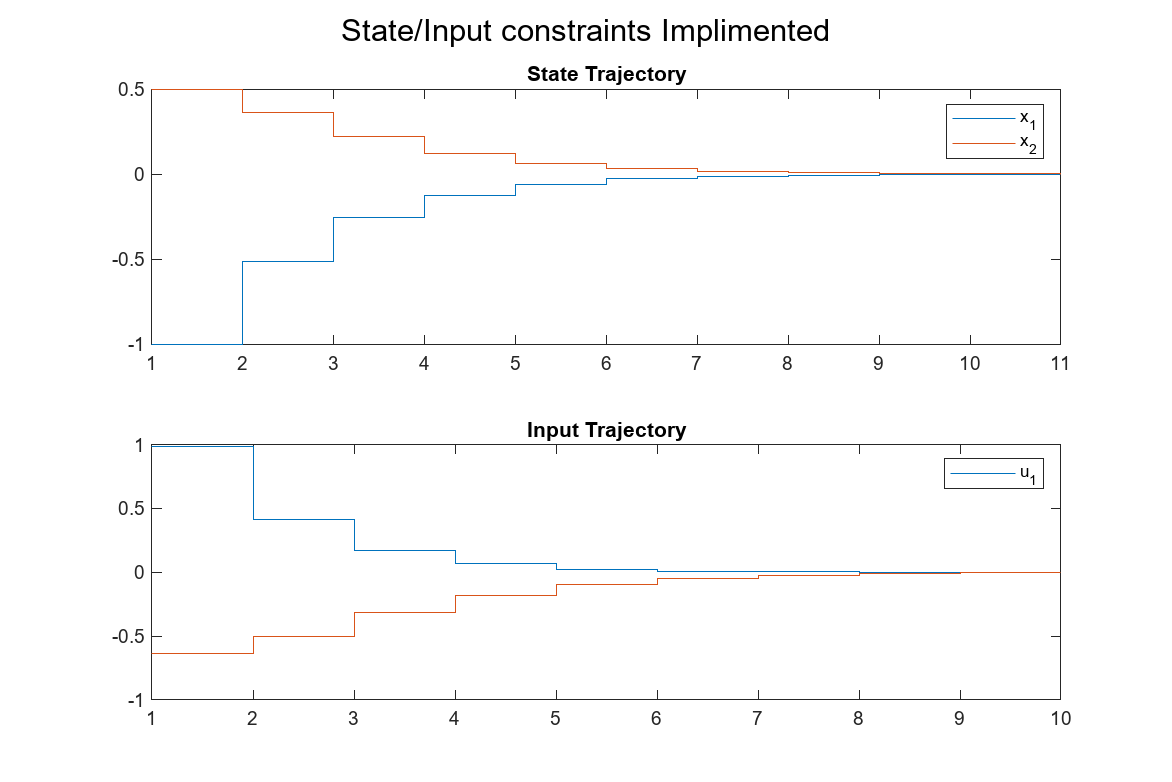
\includegraphics[width=0.7\textwidth]{figs/pblm2c}
\end{figure}

% 2d)
\newpage
\subsection{}
I had a lot of difficulty getting the batch method to work correctly (see matlab)...
The specific results requested are here:
\begin{figure}[h]
    \centering
    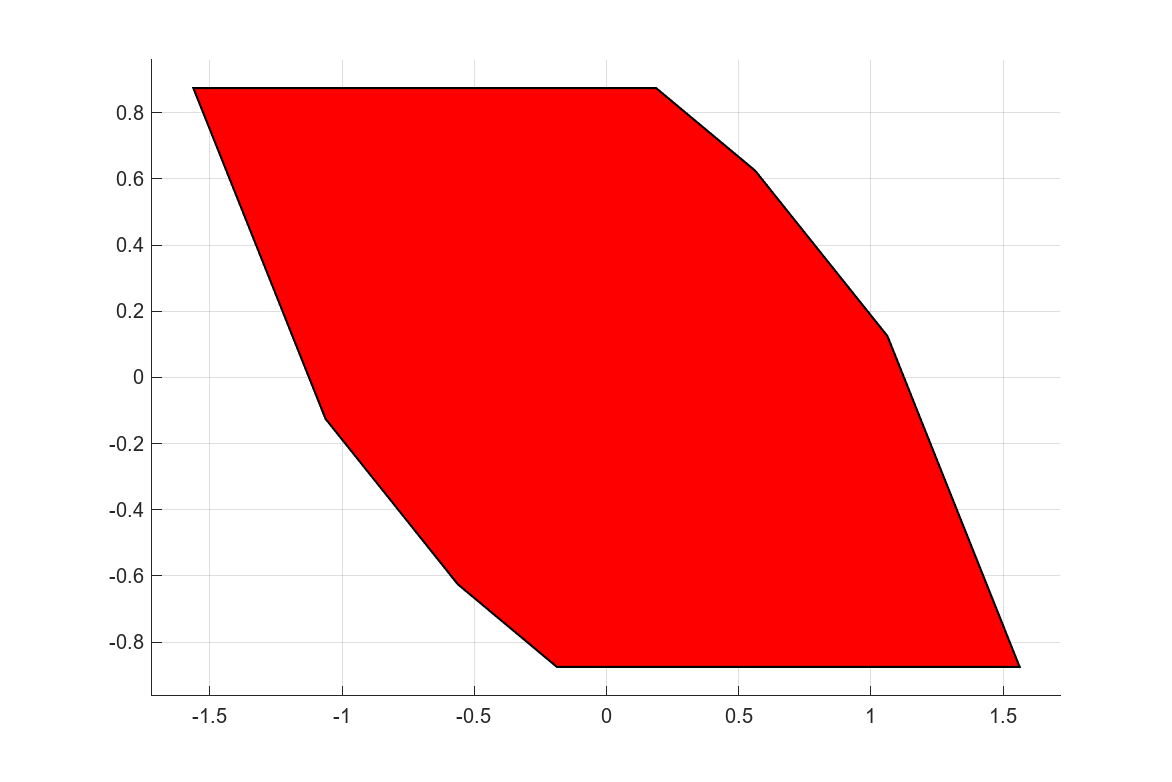
\includegraphics[width=0.7\textwidth]{figs/pblm2d.png}
\end{figure}

The recursive approach was faster as expected (0.16s vs 0.38s).


\newpage
\appendix
\section{MATLAB Files}
MATLAB files included as follows.
% 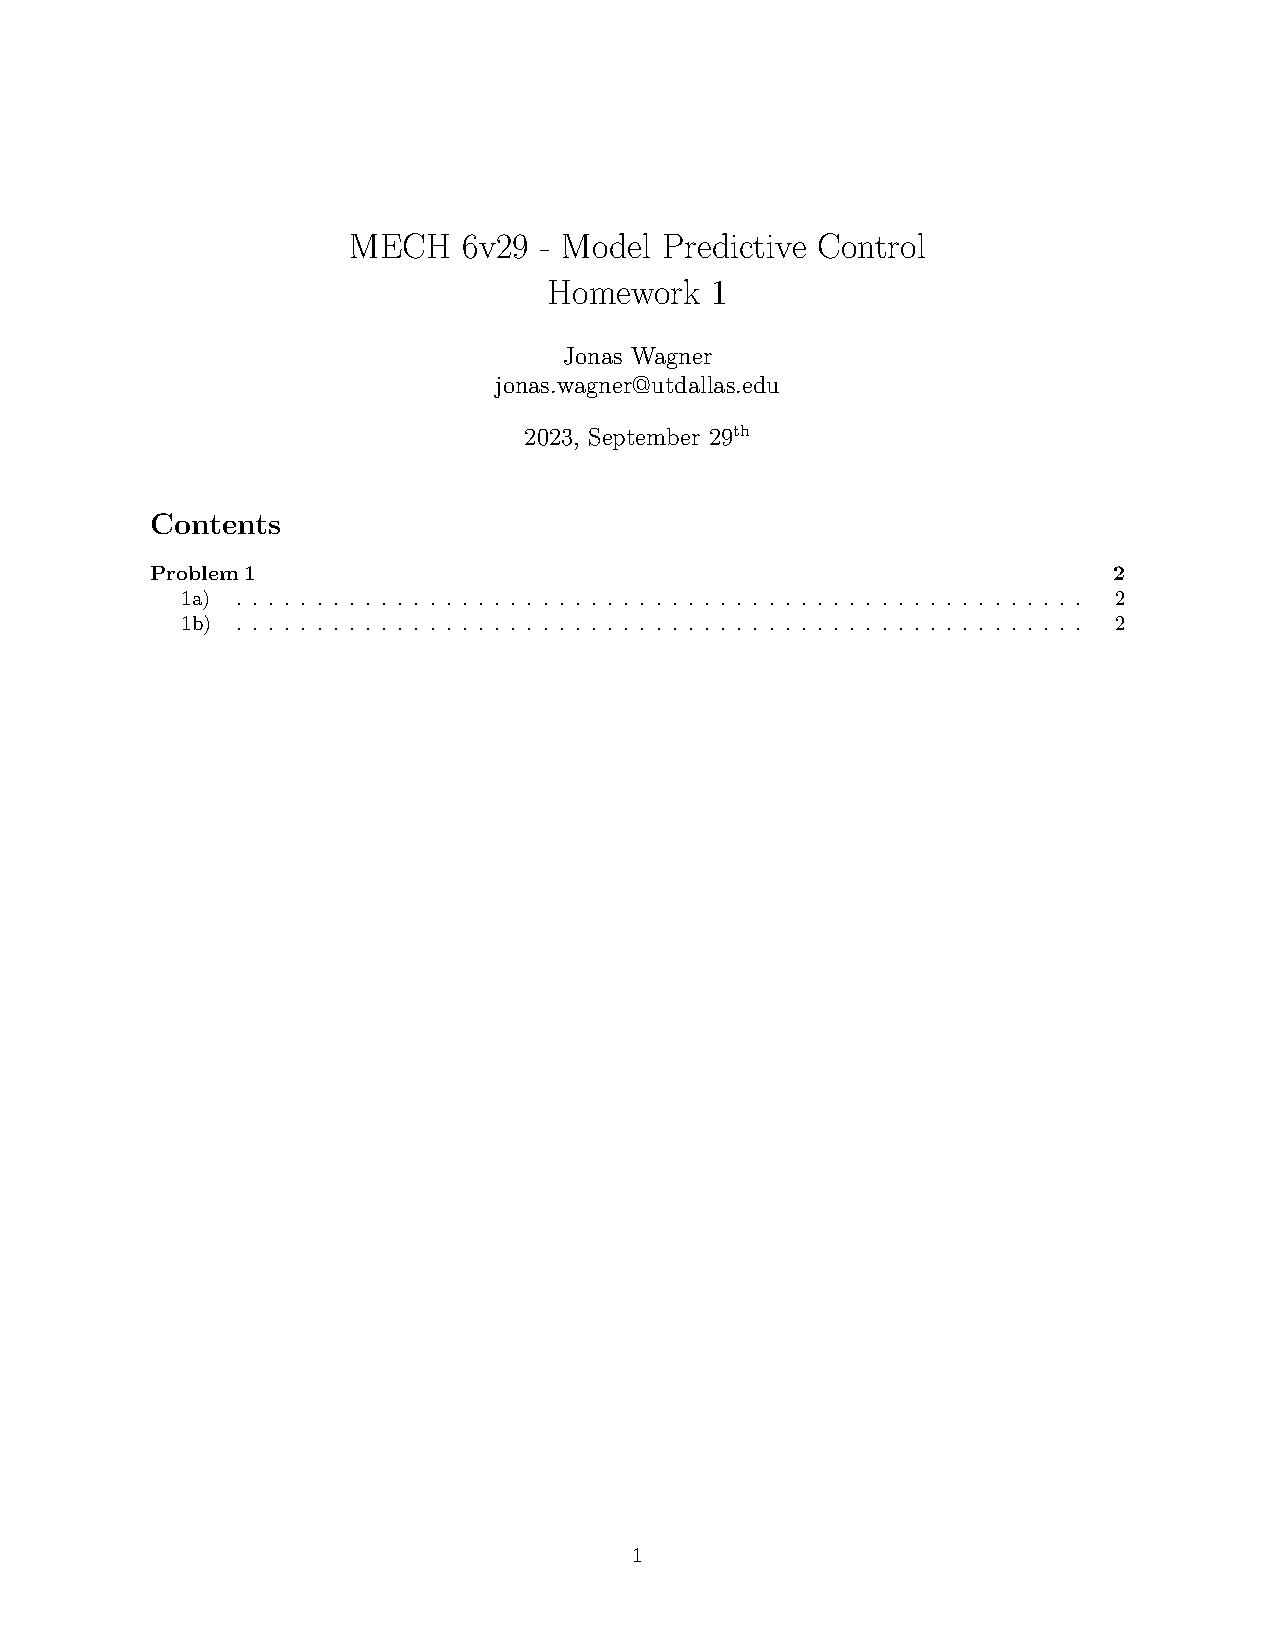
\includepdf[pages=-]{HW2.pdf}
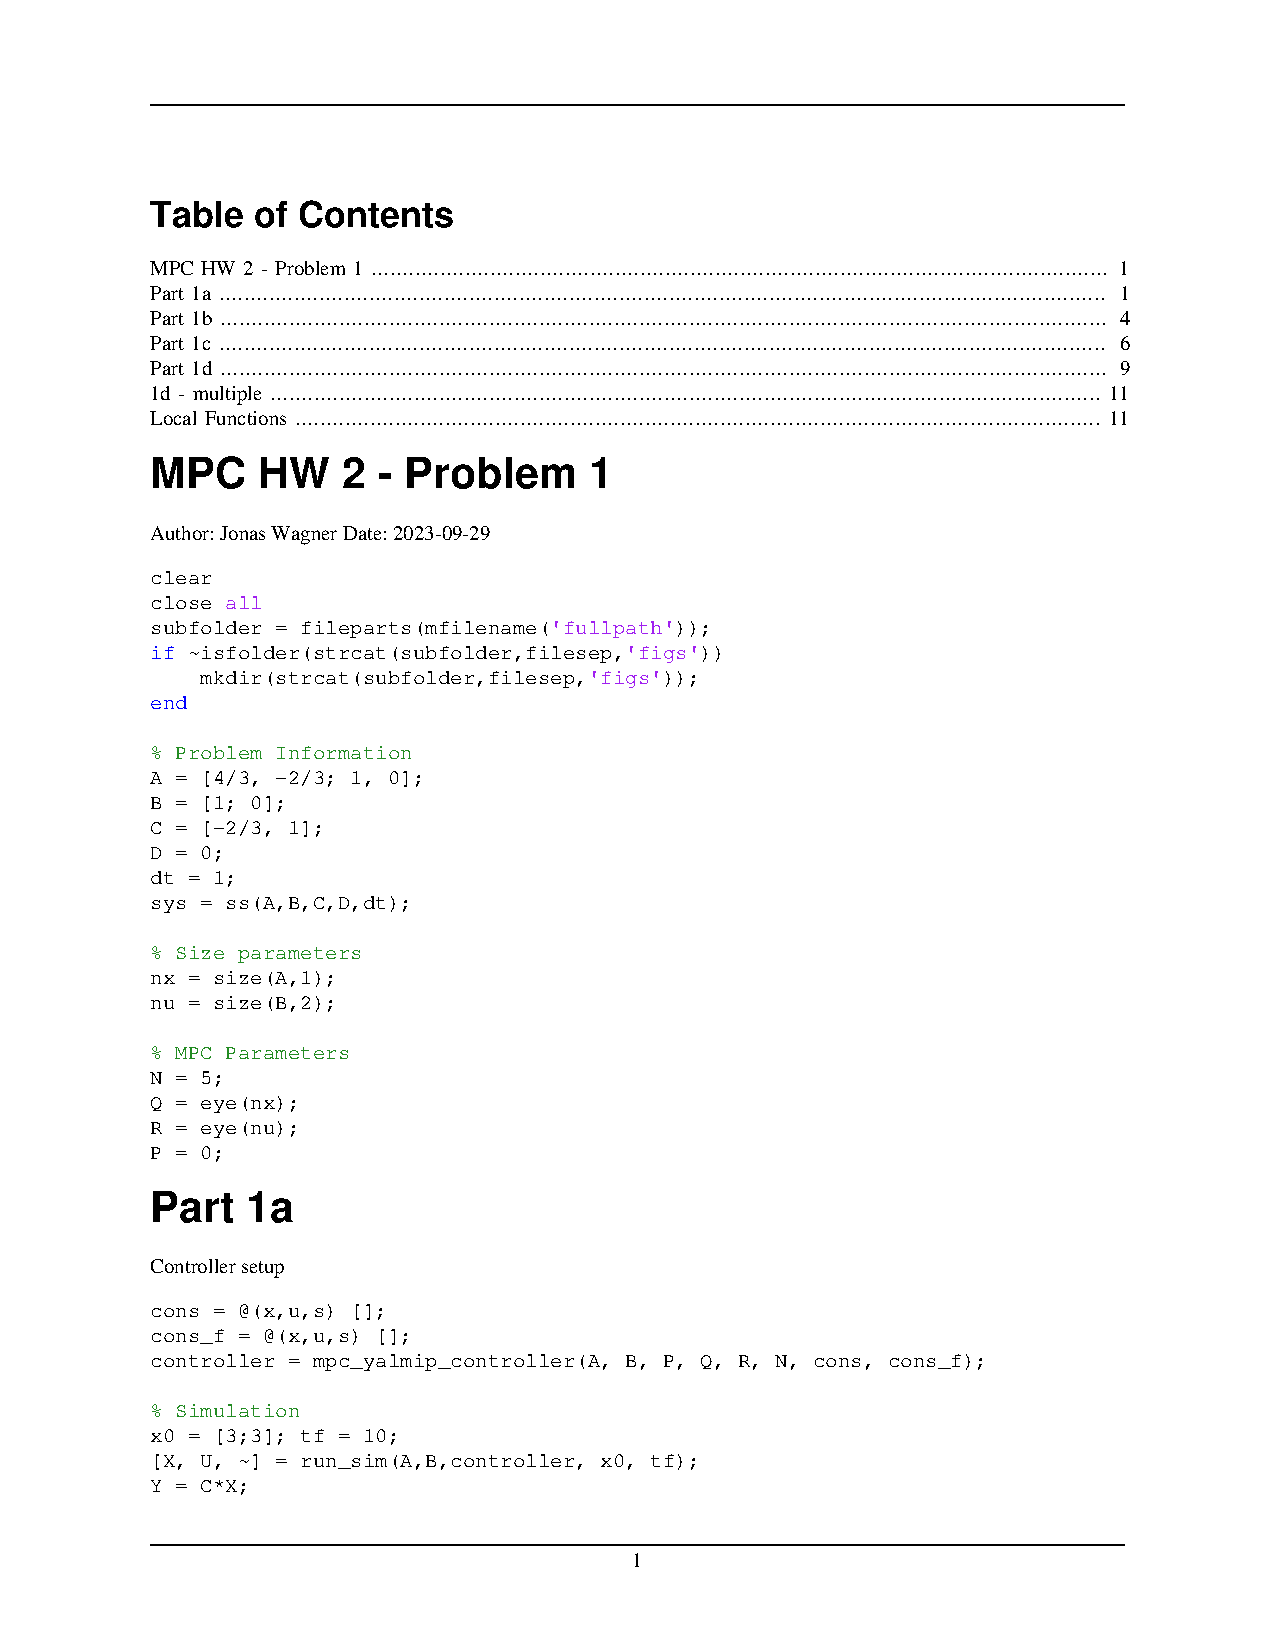
\includepdf[pages=-]{html/HW2_pblm1.pdf}
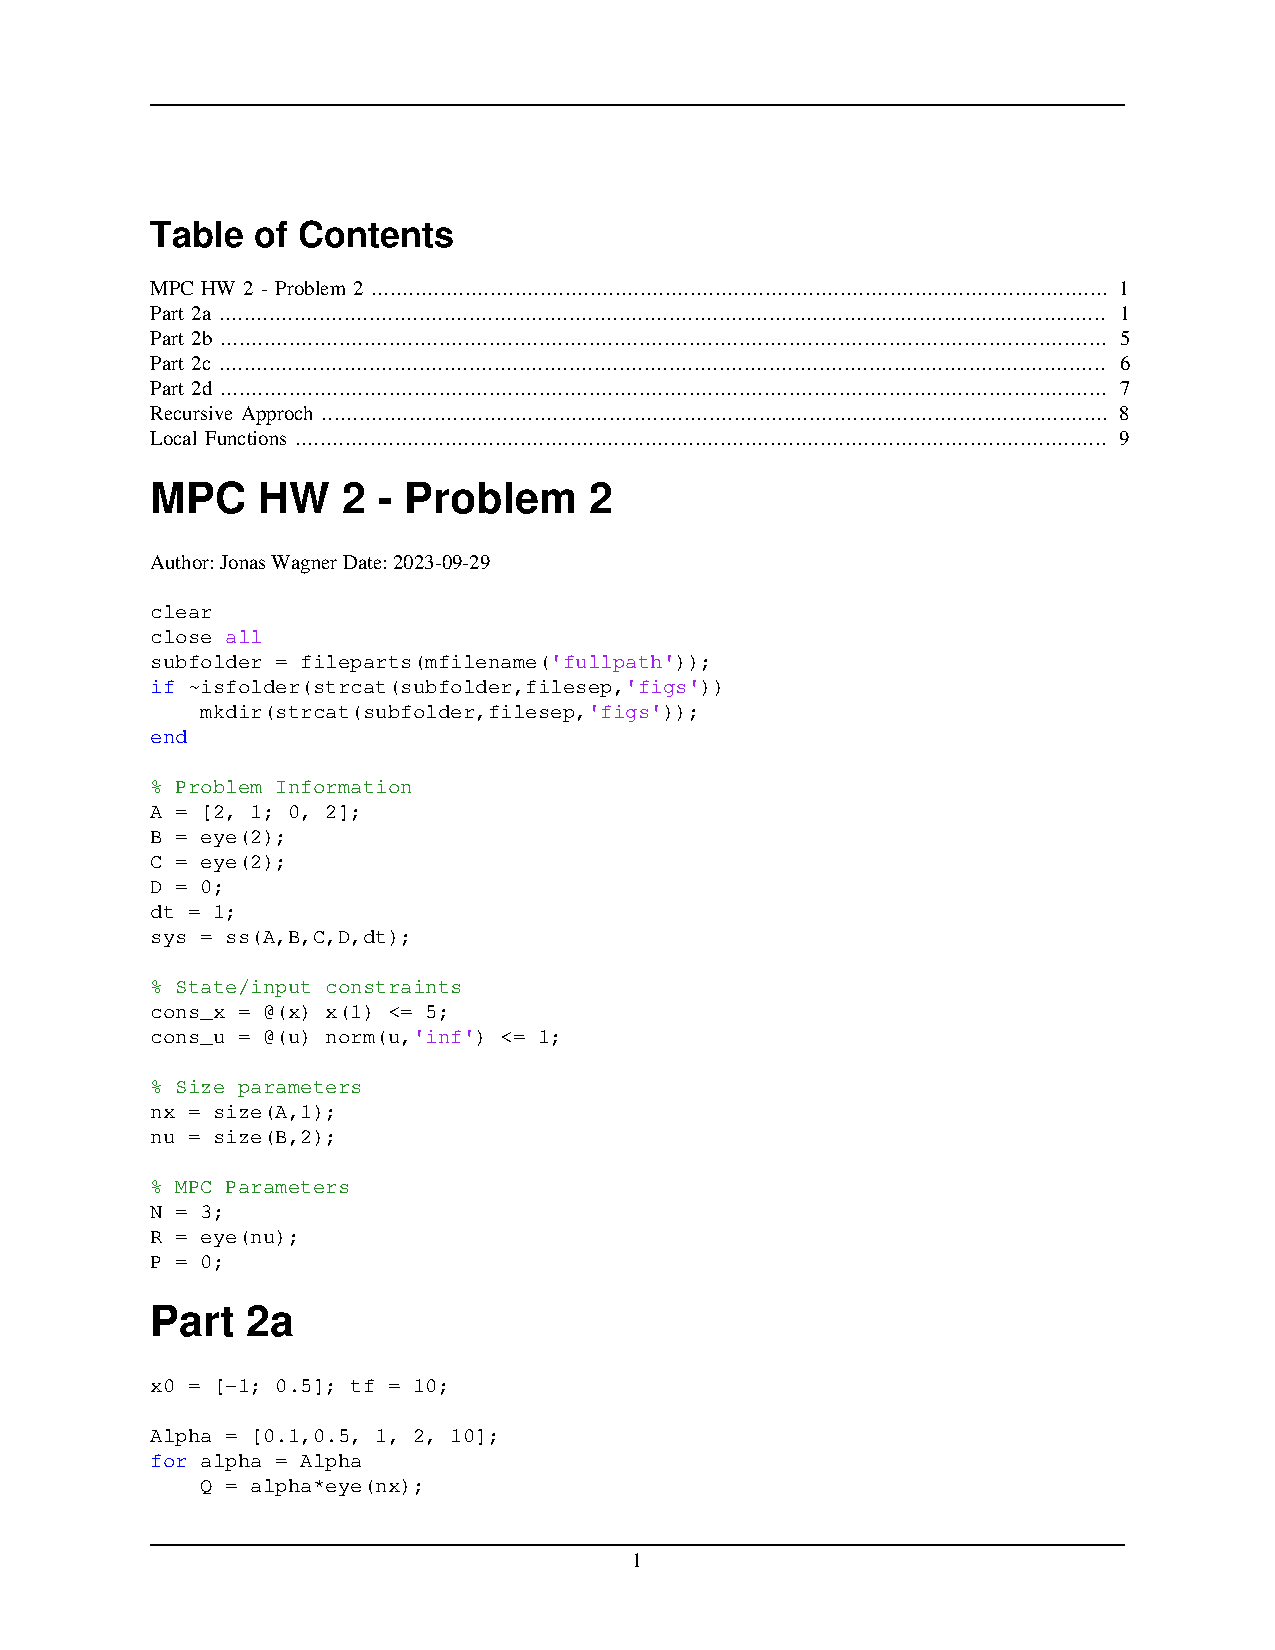
\includepdf[pages=-]{html/HW2_pblm2.pdf}


\end{document}
